\documentclass[a4paper]{exam}
\usepackage[utf8]{inputenc}
\printanswers\usepackage[utf8]{inputenc}
\usepackage[top=2in, bottom=1.25in, left=1.25in, right=1.25in]{geometry}
\usepackage{graphicx}
\usepackage{url}
\usepackage{subcaption}
\usepackage{amsmath, amsthm, amssymb}
\usepackage{epstopdf}
\usepackage{csquotes}
\usepackage{tikz}
\usepackage{placeins}
\usepackage{hyperref}
\usepackage{tikz,pgfplots}
\usepackage{listings}
\usepackage{mwe}
\usepackage{systeme}
\usepackage{cleveref}
\usepackage{qtree}

\usepackage{color}


\definecolor{codegreen}{rgb}{0,0.6,0}
\definecolor{codegray}{rgb}{0.5,0.5,0.5}
\definecolor{codepurple}{rgb}{0.58,0,0.82}
\definecolor{backcolour}{rgb}{0.95,0.95,0.92}

\lstdefinestyle{mystyle}{
    backgroundcolor=\color{backcolour},
    commentstyle=\color{codegreen},
    keywordstyle=\color{magenta},
    numberstyle=\tiny\color{codegray},
    stringstyle=\color{codepurple},
    basicstyle=\footnotesize,
    breakatwhitespace=false,
    breaklines=true,
    captionpos=b,
    keepspaces=true,
    numbers=left,
    numbersep=5pt,
    showspaces=false,
    showstringspaces=false,
    showtabs=false,
    tabsize=2
}

\lstset{style=mystyle}


\title{Homework 2 - Parallel Programming for Large Scale Problems - SF2568}
\author{Gabriel Carrizo}
\date{December 2017}

%-------------------------------------------------------
\begin{document}

\maketitle

\pagebreak
\begin{questions}

\section{Broadcast Operation}

\addpoints\question Design an algorithm for the broadcast operation only using point-to-point comunication.

\begin{solution}
The brodcast operation is an operation that sends the information of one node to all other processes. Using recursive doubling one can `spread' amongst processes, much like an infection moves through a host.

The idea is that the process with the data sends its data to another process. Once that process also possesses the data, both processes send the data to two other processes. Now we have four processes with data and all four can send data to four other processes. This procedure repeats until all processes posses the data (see figure \ref{graph}).

The complexity of the solution in parallel is dependent on the number of processors used.

See Listing \ref{lst:label} for pseudoecode. (Made under the assumption that $P=2^D$)
\end{solution}

\begin{figure}[ht!]
  \center
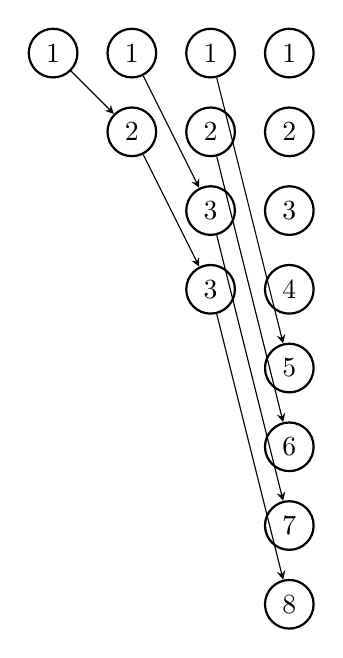
\begin{tikzpicture}
  \begin{scope}[every node/.style={circle,thick,draw}]
      \node (10) at (0,5) {1};

      \node (11) at (1,5) {1};
      \node (21) at (1,4) {2};

      \node (12) at (2,5) {1};
      \node (22) at (2,4) {2};
      \node (32) at (2,3) {3};
      \node (42) at (2,2) {3};

      \node (13) at (3,5) {1};
      \node (23) at (3,4) {2};
      \node (33) at (3,3) {3};
      \node (43) at (3,2) {4};
      \node (53) at (3,1) {5};
      \node (63) at (3,0) {6};
      \node (73) at (3,-1) {7};
      \node (83) at (3,-2) {8};
  \end{scope}

  \tikzset{thin arc/.style={->, black, fill=none, thin, >=stealth, text=black}}

  \draw[thin arc] (10) -- (21);

  \draw[thin arc] (11) -- (32);
  \draw[thin arc] (21) -- (42);

  \draw[thin arc] (12) -- (53);
  \draw[thin arc] (22) -- (63);
  \draw[thin arc] (32) -- (73);
  \draw[thin arc] (42) -- (83);

\end{tikzpicture}
\caption{Graph representation of broadcasting with recursive doubling for $P = 8$.}
\label{graph}
\end{figure}

\pagebreak
\lstinputlisting[style=mystyle,caption={Pseudocode for broadcasting operation.},label={lst:label},language=Python]{scripts/broadcast.py}

\addpoints \question Do a (time-)performance analysis for your algorithm.

\begin{solution}
  For this implementation we are looking at:

  Local computation time:

  $t_{comp,1} = 1t_a$ (where $t_a$ is the time for one basic operation) for allocating memory for x.

  Recursive doubling step:

  $t = D(t_{startup} + w_pt_{data} + 3t_a) = \log P(t_{startup} + wt_{data} + 3t_a)$

  Where $3t_a$ is from the (at most) two if statement evaluations and the computation of the destination.

  Total computation time:

  $T_p = t_{comp,1} + t = t_a + \log P(t_{startup} + wt_{data} + 3t_a)$
\end{solution}

\addpoints \question How can the scatter operation be implemented using $O(log P)$ communication steps?

\begin{solution}
You could broadcast the data and have each process select its portion of the data, however this would result in high memory overhead.

A solution to this is that the ground process sends the upper half the data to the middle node by performing the bitflip in reverse, from highest bit to lowest bit. This way, if memory management is done properly there wont be any memory overhead. (See figure \ref{graph_2})
\end{solution}

\begin{figure}[ht!]
  \center
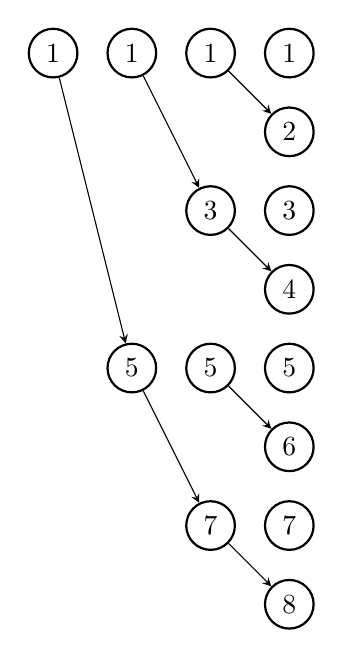
\begin{tikzpicture}
  \begin{scope}[every node/.style={circle,thick,draw}]
      \node (10) at (0,5) {1};

      \node (11) at (1,5) {1};
      \node (51) at (1,1) {5};

      \node (12) at (2,5) {1};
      \node (32) at (2,3) {3};
      \node (52) at (2,1) {5};
      \node (72) at (2,-1) {7};

      \node (13) at (3,5) {1};
      \node (23) at (3,4) {2};
      \node (33) at (3,3) {3};
      \node (43) at (3,2) {4};
      \node (53) at (3,1) {5};
      \node (63) at (3,0) {6};
      \node (73) at (3,-1) {7};
      \node (83) at (3,-2) {8};
  \end{scope}

  \tikzset{thin arc/.style={->, black, fill=none, thin, >=stealth, text=black}}

  \draw[thin arc] (10) -- (51);

  \draw[thin arc] (11) -- (32);
  \draw[thin arc] (51) -- (72);

  \draw[thin arc] (12) -- (23);
  \draw[thin arc] (32) -- (43);
  \draw[thin arc] (52) -- (63);
  \draw[thin arc] (72) -- (83);

\end{tikzpicture}
\caption{Graph representation of scatter with recursive doubling for $P = 8$.}
\label{graph_2}
\end{figure}

\section{Transpose}
\begin{solution}
  Assuming that what the algorithm from class leaves us with a grid with load balanced data distribution where each process has address $P[row,col]$:

  \begin{equation*}
    M =
    \begin{bmatrix}
      y_0 & y_0 & ... & y_0 \\
      y_1 & y_1 & ... & y_1 \\
      ... & ... & ... & ... \\
      y_P & y_P & ... & y_P
    \end{bmatrix}
  \end{equation*}

  Which we want to transpoe into:

\begin{equation*} M^T =
  \begin{bmatrix}
    y_0 & y_1 & ... &y_P\\
    y_0 & y_1 & ... &y_P\\
    ... & ... & ... &...\\
    y_0 & y_1 & ... &y_P
  \end{bmatrix}
\end{equation*}

There are two approaches that work with the broadcast algorithm suggested in the previous section.

The first one is to send the data from the first column to the first row, such that P[0,1] sends to P[1,0], P[0,2] send to P[2,0], etc. Once the first row is filled with its initial value the broadcast be performed, just like in the previous section but for each column individually.

The second approach I will suggest is to perform a cyclic shift for the rows of each column s.t. every diagonal element is shifted to the the first row of matrix M. This method requires some adjustments so the processes send and recieve to and from the correct index (see Listing \ref{lst:transpose})

The first approach requires an extra communication step and will also require sending data to some processes on the diagonal that already posses the data. The second approach requires some extra computation steps but should overall be quicker since it requires fewer communication steps.
\end{solution}

\lstinputlisting[caption={Pseudocode for transpose with the broadcast operation operation.},label={lst:transpose},language=Python]{scripts/transpose.py}

\addpoints \question Performance analysis:

The first approach would require an additional communication step in the beginning which would result in the following performance:

$T_p = t_{comp,1} + t = t_a + \log P(t_{startup} + wt_{data} + 3t_a) + t_{startup} + t_{data}$

The second approach (seen in psuedocode in Listings \ref{lst:transpose}) would add one additional computation for the cyclic shifts of the process address and the recipient address. Luckily, this approach requires just as many communication steps as the broadcast approach in section 1.

$t_{comp,1} = 4t_a$

Recursive doubling:

$t = \log P(t_{startup} + wt_{data} + 6t_a)$

Total:

$T_P = t_{comp,1} + t = 4t_a +\log P(t_{startup} + wt_{data} + 6t_a) $

\section{Solving DE with Poisson - Jacobi Iterations}

In this section the data was linearly distributed over the processes. Each process would need the results of its neighbouring processes and this problem was solved using red-black communication. This procedure ensures that all processes communicate with each other in the correct order such that there is no deadlocking.

In the code, red-black communication looks like this:

\lstinputlisting[caption={Red-black communication.},label={lst:label},language=C]{scripts/redblack.c}

Before the implementation could begin functions $f(x)$ and $r(x)$ were computed such that:
\begin{equation}
  f(x) = u'' - r(x)u
\end{equation}
and
\begin{equation}
  r(x) \leq 0 \; \forall \; x \; \epsilon \; [0,1]
\end{equation}

with a $u$ that satisfies the boundary conditions:

\begin{equation}
  u(0) = u(1) = 0
\end{equation}

\begin{equation*}
  u(x) = x(x-1)
\end{equation*}

Which gives us the following $f(x)$:

\begin{equation}
  f(x) = 2 - x^2(x-1)
\end{equation}

The following result was obtained for $1e6$ iterations on 8 processors:

\begin{figure}
  \center
  \includegraphics[width=0.7\linewidth]{plots/u_plot.png}
  \caption{Output generated from our poisson equation solver generated by jacobi iterations compared to true solution.}
  \label{plot}
\end{figure}


\end{questions}
\end{document}
